\documentclass[12pt]{article}


\usepackage{amssymb}
\usepackage{amsmath}
\usepackage{fullpage}
\usepackage{epsfig}
\usepackage{epstopdf}
\everymath{\displaystyle}
\usepackage{enumerate}

\newif\ifans

\anstrue

\begin{document}

\begin{center}
\underline{\LARGE{Chapter 3.6: Limits \& Continuity of Trig. Functions}}
\end{center}

\subsection*{Expected Skills:}

\begin{itemize}

\item Know where the trigonometric functions are continuous and be able to evaluate basic trigonometric limits.

\item Be able to use $\lim_{x\rightarrow0}\frac{\sin{x}}{x}=1$ or $\lim_{x \rightarrow 0}\frac{1-\cos{x}}{x}=0$ to help find the limits of functions involving trigonometric expressions, when appropriate.

\item Understand the squeeze theorem and be able to use it to compute certain limits.

\end{itemize}

\subsection*{Practice Problems: }

\noindent {\bf Evaluate the following limits using the squeeze theorem.}

\begin{enumerate}

\item Let $f(x)$ be a function which satisfies $\displaystyle 5x-6 \leq f(x) \leq x^2+3x-5$ for all $x \geq 0$.  Compute $\displaystyle \lim_{x \rightarrow 1}{f(x)}$.

\ifans{\fbox{$-1$}} \fi

\item $\lim_{x\to\infty} \frac{x+\cos{x}}{3x+1}$

\ifans{\fbox{\parbox{1\linewidth}{Notice that $f(x)=\frac{x+\cos{x}}{3x+1}$ can be bounded as follows: $$\frac{x-1}{3x+1} \leq \frac{x+\cos{x}}{3x+1} \leq \frac{x+1}{3x+1}$$  Since $\lim_{x\to\infty} \frac{x-1}{3x+1}=\lim_{x\to\infty}  \frac{x+1}{3x+1}=\frac{1}{3}$, it follows that $\lim_{x\to\infty}  \frac{x+\cos{x}}{3x+1}=\frac{1}{3}$.}}} \fi

\end{enumerate}


\noindent {\bf For problems 3-19, evaluate the given limit.  If a limit does not exist, write DNE, $+\infty$, or $-\infty$ (whichever is most appropriate).}

\begin{enumerate}
\setcounter{enumi}{2}

\item  $\displaystyle \lim_{x\rightarrow \frac{\pi}{4}} \sin{(2x)}$ 

\ifans{\fbox{1}} \fi

\item $\displaystyle \lim_{\theta \rightarrow \pi}{(\theta \cos{\theta})}$

\ifans{\fbox{$-\pi$}} \fi

\item  $\displaystyle \lim_{x\rightarrow 0^+} \csc x$ 

\ifans{\fbox{$+\infty$}} \fi

\item  $\displaystyle \lim_{x\rightarrow \frac{\pi}{2}^+} \tan x$ 

\ifans{\fbox{$-\infty$}} \fi

\item  $\displaystyle \lim_{x\rightarrow \frac{\pi}{2}^-} \tan x$ 

\ifans{\fbox{$+\infty$}} \fi

\item $\displaystyle \lim_{x \rightarrow \frac{\pi}{4}}{\sec{x}}$

\ifans{\fbox{$\sqrt{2}$}} \fi

\item $\displaystyle \lim_{x\rightarrow 0}{\left(\frac{\sin{x}}{3x}\right)}$ 

\ifans{\fbox{$\displaystyle \frac{1}{3}$}} \fi

\item $\displaystyle \lim_{x\rightarrow 0}{\left(\frac{\sin{3x}}{3x}\right)}$ 

\ifans{\fbox{$\displaystyle 1$}} \fi

\item $\displaystyle \lim_{x\rightarrow 0}{\left(\frac{\sin{x}}{|x|}\right)}$

\ifans{\fbox{DNE}} \fi

\item $\displaystyle \lim_{x\rightarrow 0}{\left(\frac{1-\cos{x}}{4x}\right)}$

\ifans{\fbox{$0$}} \fi

\item $\displaystyle \lim_{x\rightarrow 0^-}{\left(\frac{\cos x}{x}\right)}$ 

\ifans{\fbox{$-\infty$}} \fi

\item $\displaystyle \lim_{x\rightarrow 0}{\left(\frac{\sin 2x}{x}\right)}$

\ifans{\fbox{2}} \fi

\item $\displaystyle \lim_{x\rightarrow 0}{\left(\frac{\tan 2x}{x}\right)}$

\ifans{\fbox{2}} \fi

\item $\displaystyle \lim_{x\rightarrow 0}{\left(\frac{1-3\cos{x}}{3x}\right)}$

\ifans{\fbox{DNE}} \fi

\item $\displaystyle \lim_{x\rightarrow 0}{\left(\frac{3x^2}{1-\cos^2{x}}\right)}$

\ifans{\fbox{3}} \fi

\item $\displaystyle \lim_{x \rightarrow 0}{\left(\frac{\tan{5x}}{\sin{9x}}\right)}$

\ifans{\fbox{$\displaystyle \frac{5}{9}$}} \fi

\end{enumerate}

\noindent {\bf For problems 19-20, evaluate the given limit by making an appropriate substitution (change of variables).  If a limit does not exist, write DNE, $+\infty$, or $-\infty$ (whichever is most appropriate).}

\begin{enumerate}
\setcounter{enumi}{18}

\item $\displaystyle \lim_{x\to 8}\frac{\sin(x-8)}{x^2-64}$

\ifans{\fbox{$\frac{1}{16}$}} \fi

\item $\displaystyle \lim_{x\to \infty}x\sin\left(\frac{2}{x}\right)$

\ifans\fbox{2}\fi

\end{enumerate}

\noindent {\bf For problem 21-23, determine the value(s) of $x$ where the given function is continuous.} 

\begin{enumerate}
\setcounter{enumi}{20}

\item $f(x) = \csc{x}$ 

\ifans{\fbox{$f(x)$ is continuous for all $x \neq \pi k$, where $k$ is any integer.}} \fi

\item $\displaystyle f(x) = \frac{1}{1-2\cos{x}}$ on $[0,2\pi]$ 

\ifans{\fbox{$f(x)$ is continuous for all $x$ in $[0,2\pi]$ except for $\displaystyle x=\frac{\pi}{3}$ and $\displaystyle x=\frac{5\pi}{3}$}} \fi

\item $\displaystyle f(x)=\left\{
\begin{array}{lll}
\cos{x} & \text{if} & x< \frac{\pi}{4}\\
&\\
\sin{x} & \text{if} & x\geq \frac{\pi}{4}
\end{array}\right.$

\ifans{\fbox{$f(x)$ is always continuous.}} \fi

\item Find all non-zero value(s) of $k$ so that $\displaystyle f(x)=\left\{\begin{array}{lll}
\frac{3\sin{(kx)}}{x} & \text{if} & x>0\\
&&\\
6k^2+5x & \text{if} & x \leq 0
\end{array}\right.$
is continuous at $x=0$.

\ifans{\fbox{$\displaystyle k=\frac{1}{2}$}} \fi

\item Use the Intermediate Value Theorem to prove that there is at least one solution to $\cos{x}=x^2$ in $(0,1)$.

\ifans{\fbox{\parbox{1\linewidth}{Let $f(x)=\cos{(x)}-x^2$.  Since $f(x)$ is continuous on $(-\infty,\infty)$, it is also continuous on $[0,1]$.  Notice that $f(0)=1>0$ and $f(1)=\cos{(1)}-1<0$.  Thus, the Intermediate Value Theorem states that there must be some $c$ in $(0,1)$ such that $f(c)=0$.  i.e., there must be at least one $c$ in $(0,1)$ such that $\cos(c)-c^2=0$ $\implies$ $\cos{(c)}=c^2$, as desired.}}} \fi


\item Let $x$ be a fixed real number.  Compute $\lim_{h \rightarrow 0}\frac{\sin{(x+h)}-\sin{x}}{h}$.  (Hint: The identity $\sin{(A+B)}=\sin{A}\cos{B}+\cos{A}\sin{B}$ will be useful.)

\ifans{\fbox{$\cos{x}$}} \fi


\item A \underline{Regular Polygon} is a polygon that is equiangular (all angles are equal in measure) and equilateral (all sides have the same length).  The diagram below shows several regular polygons inscribed within a circle of radius $r$.

\begin{center}

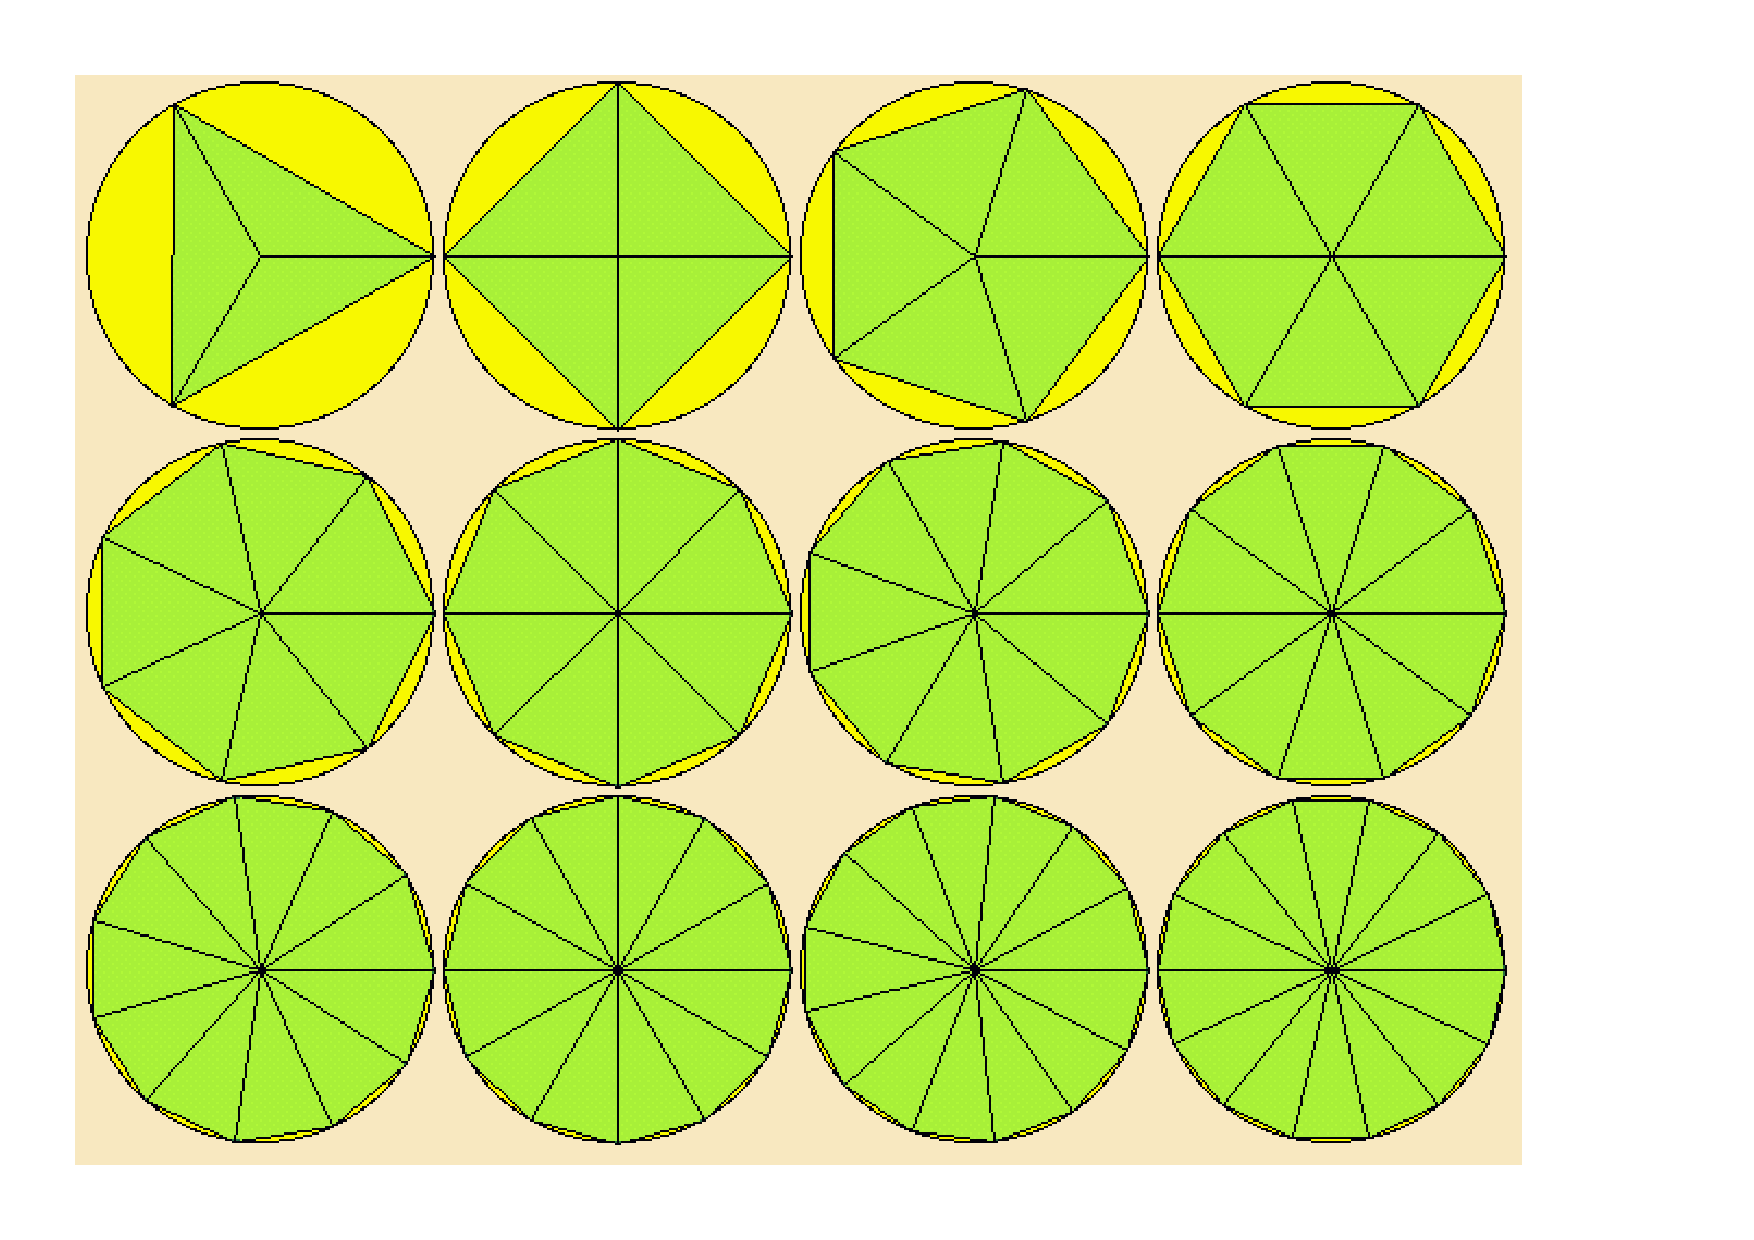
\includegraphics[scale=0.3]{Inscribed.pdf}

\end{center}

\begin{enumerate}

\item Let $A_n$ be the area of a regular $n$-sided polygon inscribed within a circle of radius $r$.  Divide the polygon into $n$ congruent triangles each with a central angle of $\frac{2\pi}{n}$ radians, as shown in the diagram above for several different values of $n$.    Show that $A_n=\frac{1}{2}r^2 \sin{\left(\frac{2\pi}{n}\right)} n$.

\ifans{\fbox{\parbox{1\linewidth}{We begin by examining one of the $n$ triangles, pictured below.
\begin{center}
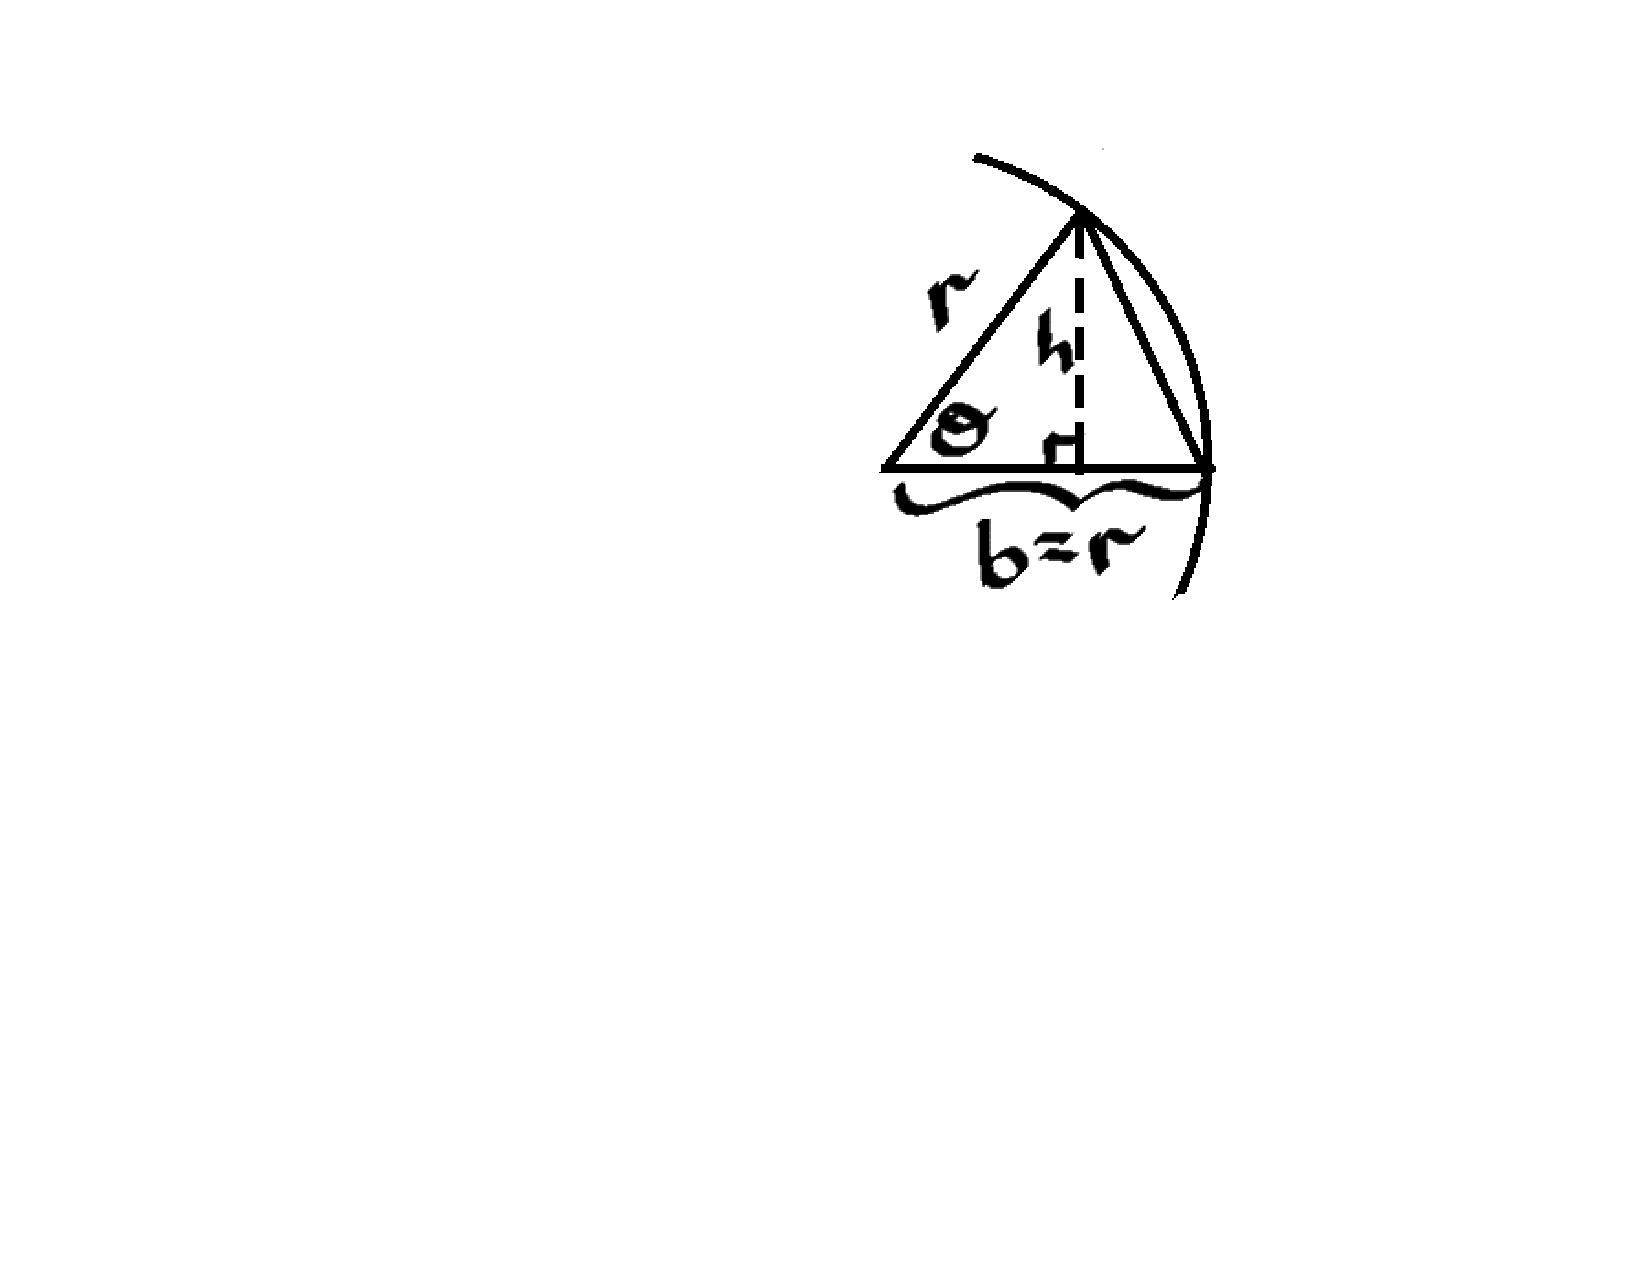
\includegraphics[scale=0.4]{triangle.pdf}
\end{center}
The base of the triangle has a length of $r$.  And, the height of the triangle is $r\sin{\theta}$, where $\theta$ is the central angle, $\frac{2\pi}{n}$.    Thus, the area of one triangle is:
$$A=\frac{1}{2}(r)\left(r\sin{\left(\frac{2\pi}{n}\right)}\right)=\frac{1}{2}r^2\sin{\left(\frac{2\pi}{n}\right)}$$
 But, the polygon is composed of $n$ such triangles.  So, the area of a regular $n$-sided polygon inscribed in the circle of radius $r$ is: 
$$A_n=\frac{1}{2}r^2\sin{\left(\frac{2\pi}{n}\right)}n$$
}}} \fi

\item What can you conclude about the area of the $n$-sided polygon as the number of sides of the polygon, $n$, approaches infinity?  In other words, compute $\lim_{n \rightarrow \infty}{A_n}$.

\ifans{\fbox{$\lim_{n \rightarrow \infty}{A_n}=\pi r^2$}} \fi

\end{enumerate}

\end{enumerate}

\end{document}